% Generated from: Zhihu/专栏：概率与统计/渐近统计 (11)：Bootstrap（上）_金鱼马_2026-07-18.md
\section{引入}

在之前的文章中，我们介绍了各种拥有渐近正态性质的统计量
\[\sqrt n(\widehat \theta_n-\theta_0)\overset{\rm d}\to\mathcal N(0,\Sigma)\]
例如在适当正则条件下的矩估计（第~\ref{ch:method-of-moments}~章）、MLE（第~\ref{ch:maximum-likelihood}~章）以及 M-估计（第~\ref{ch:m-and-z-estimation}~章）等。

一方面，当一个统计量没有渐近正态时，例如一阶退化的 U-统计量，其渐近分布会变成 χ² 分布的加权和。此时，我们可能会需要诉诸适用性更加广泛的非参数方法，例如本节将介绍的 Bootstrap。

另一方面，即使一个统计量是渐近正态的，我们依然有改进的空间------这个改进的空间是由 Peter Hall 在 90 年代初提出来的。考虑如下标准化，或称``学生化 (studentized)''的一维统计量
\[
T_n=\frac{\widehat{\theta}_n-\theta_0}{\widehat{\mathrm{se}}_n}.
\]
通常的正态近似，或称``Wald 近似''，这是说
$$P(T_n\leq x)\approx \Phi(x),\quad \text{ 当 }n\to\infty$$
对固定的 $x$ 成立，这是一个一阶的近似。在许多满足适当正则条件的问题中，这个结论还能够写作
\[P(T_n\leq x)=\Phi(x)+O(n^{-1/2})\]
上式能够捕捉极限分布的均值、方差信息。但有些时候，尤其是样本量 $n$ 不大的时候，这无法很好地刻画诸如偏度、偏差 (bias) 或者曲率 (curvature)； $O(n^{-1/2})$ 的误差会把这些信息给掩盖掉。

当然，读者可能会想到第~\ref{ch:characteristic-functions}~章中介绍的修正方法：\emph{Edgeworth 展开}（\cite{hall1992}, Theorem 2.2）。以二阶为例，对满足适当光滑条件（Cramér 条件）的统计量 $T_n$，Edgeworth 展开有形式
\[P(T_n\leq x) = \Phi(x) +\frac{1}{\sqrt{n}}p_1(x;P)\varphi(x) +\frac{1}{n}p_2(x;P)\varphi(x) +o(n^{-1})\]
其中 $\varphi$ 是标准正态密度，$p_1$ 和 $p_2$ 是依赖于 $P$ 的多项式。渐近正态仅贡献了 $\Phi(x)$ ，而后面的第一个校正项内包含了涉及三阶累积量、即偏度的信息，也包含统计量的一阶偏差和曲率；第二个校正项包含了四阶累积量、即峰度的信息，以及统计量的更高阶偏差和曲率等。

假如 $T_n$ 的性质足够好，理论上可以允许我们 Edgeworth 展开到很多阶，从而让误差的阶非常非常小。为什么这种做法很少见呢？答案是：多项式 $p_j$ 本身实在过于复杂，其系数依赖未知总体分布 $P$ 的矩、累积量 (cumulant)、 $\Phi(x)$ 的高阶导数、还有其他讨厌参数等。在某些特定问题下，低阶 Edgeworth 展开确实可以提供非常好的纠偏，但在一般问题中，Edgeworth 展开往往是无能为力的。如 MLE 或者 M-估计，推导 Edgeworth 展开的高阶项比证明渐近正态难得多。

Peter Hall 的核心观察是：可以用经验分布 $\mathbb P_n$ 来代替 $P$ ，来对校正项进行估计；Bootstrap 本质上则自动完成了这件事。

下面先简单说明机制，假设 $T_n$ 有一阶 Edgeworth 展开
\[P(T_n\leq x) = \Phi(x)+\frac{1}{\sqrt{n}}p_1(x;P)\varphi(x)+O(n^{-1})\]
如果能找到 Bootstrap 统计量 $T_n^*$ （这里的星号 * 代表条件于样本数据），并满足
\[
P^*(T_n^*\leq x) = \Phi(x)+\frac{1}{\sqrt{n}}p_1(x;\mathbb P_n)\varphi(x)+O_P(n^{-1}),
\]
并且这里的多项式 $p_1$ 满足对每个 $x$ ，
\[
p_1(x;\mathbb P_n)-p_1(x;P)=O_P(n^{-1/2}),
\]

那么两式作差，就有
\[\sup_x \left| P^*(T_n^*\leq x)-P(T_n\leq x) \right| =O_{P}(n^{-1})\]
这就体现出了高阶优势： $n^{-1/2}$ 阶修正项中的系数只需估计到 $n^{-1/2}$ 阶，两者相乘便产生 $n^{-1}$ 阶误差。这就是Bootstrap 的目标：借助数据实现自动的 Edgeworth 校正，达到比原有统计量更优的收敛速度。

还要指出的一点是，区分下面的两个概念：

\begin{itemize}
\tightlist
\item
  \textbf{\emph{一阶正确性}} (first order valid)，指的是 $\sup_x \left| P^*(T_n^*\leq x)-P(T_n\leq x) \right| \overset{P}\to 0$ ；

\begin{itemize}
  \tightlist
  \item
    它说明 Bootstrap ``是对的''：当 $n\to\infty$ 时候， $T_n^*$ 确实能够刻画 $T_n$ 的分布；但没有说明这里逼近的速度。
  \end{itemize}
\item
  \textbf{\emph{二阶准确性}} (second order accuracy)，指的是 $\sup_x \left| P^*(T_n^*\leq x)-P(T_n\leq x) \right| =O_P(n^{-1})$ ；

\begin{itemize}
  \tightlist
  \item
    这个结论不是自动成立的，需要一些更强的条件，包括统计量的光滑性、有足够阶矩等，并且要求统计量至少在渐近意义上是一个枢轴量 (pivotal)。
  \end{itemize}
\end{itemize}

这里补充定义：若一个关于样本 $X_1,\dots,X_n$ 和真实参数 $\theta$ 的函数 $G_n(X_1,\dots,X_n;\theta)$ 的分布不依赖于 $\theta$ ，则称其为枢轴量 (pivotal)；若其当 $n\to\infty$ 时的渐近分布不依赖于 $\theta$ ，则称作渐近枢轴量。这里允许枢轴量作为 $\theta$ 的函数，但当说``某某统计量是 (渐近) 枢轴量''时，意味着这个统计量不含未知参数，且其 (渐近) 分布已知。

\section{非参数 Bootstrap}

\subsection{基本算法}

设 $X_1,\ldots,X_n\sim P$ 是取值于 $\mathscr X$ 的 i.i.d. 样本，记经验分布为 $\mathbb P_n=\frac{1}{n}\sum_{j=1}^n\delta_{X_j}$。我们用经验分布构造所谓``插入估计 (plug-in estimators)''：若我们对概率测度 $P$ 的某个泛函 $\theta_0=\theta(P)$ 感兴趣，那么利用 $\mathbb P_n\approx P$，将 $\mathbb P_n$ ``插入''到泛函中，得到 $\widehat\theta_n=\theta(\mathbb P_n)$ 作为 $\theta_0$ 的估计（见第~\ref{ch:u-statistics}~章）。

Bootstrap 的核心做法和``插入估计''类似：既然 $P$ 是未知的，那么在所有需要用到未知 $P$ 的地方，都用 $\mathbb P_n$ 替代。而既然 $\mathbb P_n$ 能``当作''真实分布，我们可以继续从其中抽样：
\[
X_1^*,\ldots,X_n^* \ \big|\  X_1,\ldots,X_n \sim \mathbb P_n\quad\text{i.i.d.}
\]

即，已有样本中独立、有放回地重新抽取。定义 Bootstrap 经验分布为
\[ \mathbb P_n^*=\frac{1}{n}\sum_{j=1}^n\delta_{X_j^*} \]以及 Bootstrap 统计量定义为 $\widehat{\theta}_n^*=\theta(\mathbb P_n^*)$ 。

实际算法如下：

\begin{enumerate}
\def\labelenumi{\arabic{enumi}.}
\tightlist
\item
  从原始样本 $X_1,\dots,X_n$ 中独立、有放回地抽取 $n$ 个观测，得到一组 Bootstrap 样本。
\item
  在该 Bootstrap 样本上计算 $\widehat{\theta}_n^*$。
\item
  重复前两步 $B$ 次，得到 $\widehat{\theta}_n^{*(1)},\ldots,\widehat{\theta}_n^{*(B)}$。
\item
  用这些重复值的经验分布近似所需的抽样分布。
\end{enumerate}

在 Bootstrap 中， $\mathbb P_n$ 总体扮演了 $P$ 的角色，因此 $\widehat{\theta}_n=\theta(\mathbb P_n)$ 也将扮演真实参数 $\theta_0$ 的角色；同时， $\mathbb P_n^*$ 则替代了原来的 $\mathbb P_n$。三者之间的对应关系如图~\ref{fig:ch11:bootstrap-principle} 所示。

\begin{figure}[htbp]
  \centering
  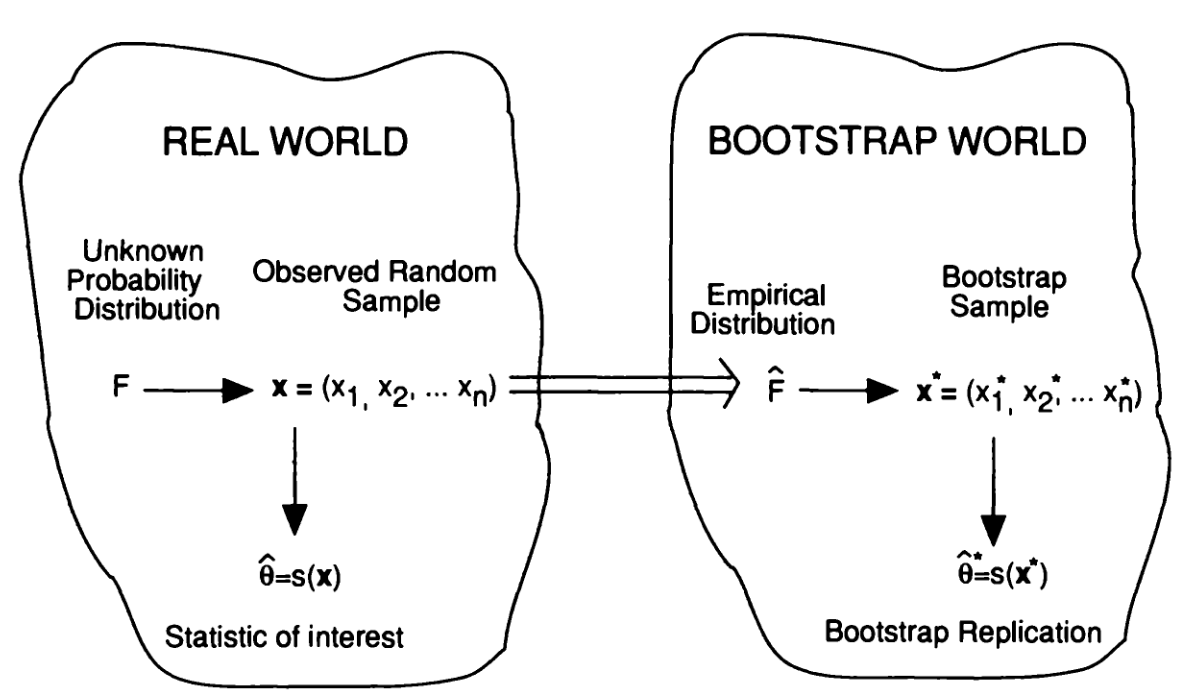
\includegraphics[width=0.88\textwidth]{figures/11-bootstrap-principle.png}
  \caption{Bootstrap 中总体、经验分布与重抽样经验分布的对应。图片来自 \cite{efrontibshirani1993}, p.~91}
  \label{fig:ch11:bootstrap-principle}
\end{figure}

Peter Hall 将此称作``俄罗斯套娃原则''，如图~\ref{fig:ch11:russian-doll-principle} 所示。

\begin{figure}[htbp]
  \centering
  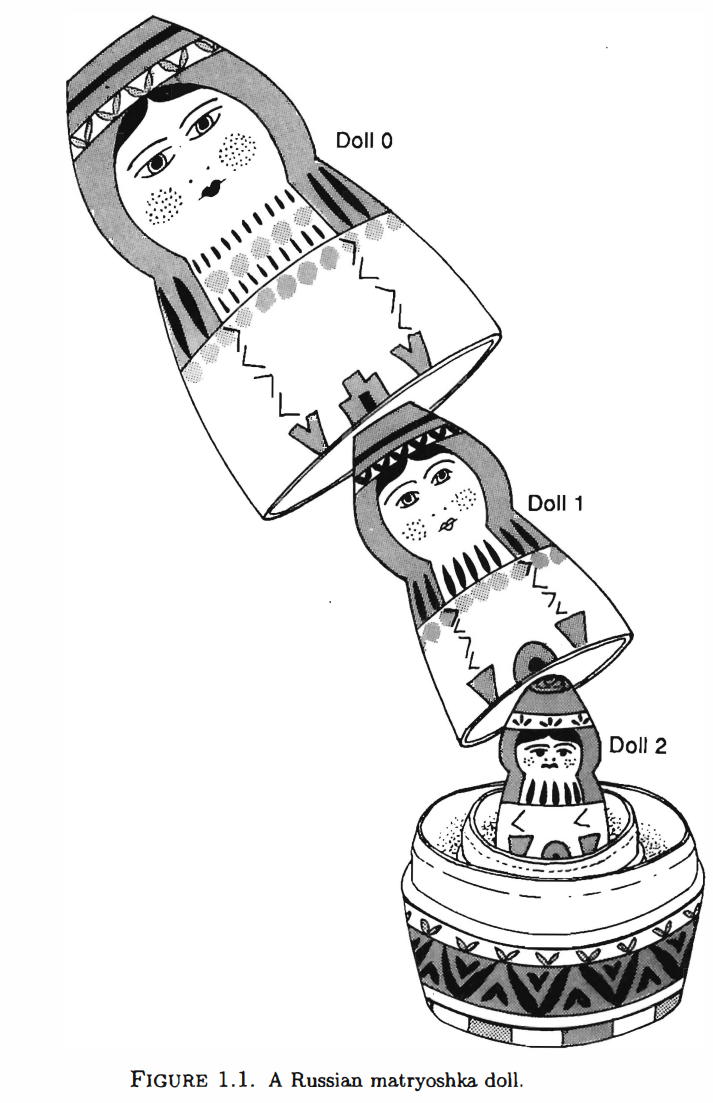
\includegraphics[height=0.68\textheight]{figures/11-russian-doll-principle.png}
  \caption{Bootstrap 的俄罗斯套娃原则。图片来自 \cite{hall1992}, p.~5}
  \label{fig:ch11:russian-doll-principle}
\end{figure}

基于上述原则，当我们想要模拟 $\sqrt{n}(\widehat{\theta}_n-\theta_0)$ 时，需要使用 $\sqrt n\big(\widehat{\theta}_n^*-\widehat{\theta}_n\big)$ 来进行刻画。

\begin{remark}

\begin{itemize}
\tightlist
\item
  理论上，如果统计量足够光滑，我们可能在上述算法基础上继续套一层，做``套娃的套娃''；但一般来讲这种做法意义不大，套一次就已足够。
\item
  上文中独立、有放回地重新抽取的样本 $X_1^*,\dots,X_n^*$ 数目仍然为 $n$ ，这里没有什么特别的原因，我们也可以非常自由地选择重抽样样本数：可以是某 $m$ ，也可以让 $m=m_n$ 随 $n$ 变化。但是 $m=n$ 是最常用的选择，对于我们后面要证明的结论也都足够。
\item
  注意到，理论中的 $P^*$ 是给定数据后的精确条件分布，而 Bootstrap 算法里是在用有限次重抽样近似它。记
  \[
  \widehat F_B^*(x)=\frac1B\sum_{b=1}^B
  \mathbb I(\widehat\theta_n^{*(b)}\leq x).
  \]
  则总误差可分解为
  \[
  \begin{aligned}
  \widehat F_B^*(x)-P(\widehat\theta_n\leq x)
  &=\left(\widehat F_B^*(x)-P^*(\widehat\theta_n^*\leq x)\right)\\
  &\quad+\left(P^*(\widehat\theta_n^*\leq x)-P(\widehat\theta_n\leq x)\right).
  \end{aligned}
  \]
  第一项是 Monte Carlo 误差，通常有 $B^{-1/2}$ 量级；第二项是 Bootstrap 方法本身的统计逼近误差。增加重复次数 $B$ 即可减少前者，因此在理论分析中，我们只关注 $P^*(\widehat\theta_n^*\leq x)-P(\theta_n\leq x)$ 这一项在 $n\to\infty$ 时的误差阶。如果能得到这项的阶，也可以帮助我们反过来确定 $B$ ，使得 Monte Carlo 误差与 Bootstrap 误差大概同阶。
\end{itemize}
\end{remark}

Bootstrap 是一个很直观很好用的办法，但是理论的建立并不容易，一般高阶刻画都比较难。我们接下来从一些更偏理论的角度，来对 Bootstrap 进行简单考察。

\subsection{条件弱收敛的补充}

本节补充部分``取条件版本''的若干概念和定理。这些细节主要用于保证在取条件时随机收敛概念严谨；读者可以略过，在后文中只需简单理解为``给定数据后的条件分布趋近于目标分布''即可。

\begin{definition*}[条件依概率收敛与条件弱收敛]
设 $Y_n$ 是样本空间 $(\Omega,\mathscr F,P)$ 中条件于给定 $\sigma$-代数 $\mathscr G_n$ 的一维统计量，后文 $\mathbb E[\ \cdot \mid \mathscr G_n]$、$P(\ \cdot\mid \mathscr G_n)$ 和条件独立等均视作某个正则条件分布的同一版本。

\begin{itemize}
\tightlist
\item
  \textbf{条件依概率收敛} 若 $Y$ 是定义于同一样本空间的随机变量，且对任意 $\epsilon>0$ ，都有 $P(|Y_n-Y|>\epsilon \mid \mathscr G_n)\overset{ P}\to 0$ ，则称 $Y_n\overset{P|\mathscr G_n}\to Y$ (依概率成立)。
\item
  \textbf{条件弱收敛} 若 $P(Y_n\le t\mid \mathscr G_n)\overset{P}\to P(Y\le t)$ ，对每个 $P(Y\le t)$ 的连续点 $t$ 成立，则称 $Y_n\overset{\rm d|\mathscr G_n}\to Y$ (依概率成立)。
\end{itemize}
\end{definition*}

\begin{remark}

\begin{itemize}
\tightlist
\item
  上面的全部 $\overset{P}\to 0$ 可以替换成 $\overset{\text{a.s.}}\to 0$ ，对应的结论替换为 a.s. 成立。
\item
  在更一般的情形，我们用\emph{有界 Lipschitz 度量}进行刻画条件弱收敛：设 $(M,d)$ 是某可分度量空间，\[ \mathrm{BL}_1(M):=\Big\{f:M\to\mathbb R:\sup_{z\in M}|f(z)|\le 1,\ |f(z_1)-f(z_2)|\le d(z_1,z_2),\ \forall z_1,z_2\in M\Big\} \]那么对 $M$ 上的两个 Borel 测度 $P,Q$ ，定义二者的有界 Lipschitz 度量为
  $$d_{\mathrm{BL}_1}(P,Q)=\sup_{f\in\mathrm{BL}_1(M)}\left|\int_Mf\mathrm dP-\int_M f\mathrm dQ\right|$$
  当一族概率测度 $\{P_n\}$ 满足 $d_{\mathrm{BL}_1}(P_n,P)\to 0$ 依概率/a.s. 收敛时，我们便称 $P_n\overset{\rm d}\to P$ 依概率/a.s. 成立。见 \cite[1.12 节]{vandervaartwellner1996}。% van de Vaart \emph{Weak Convergence and Empirical Processes} 的 1.12。
\end{itemize}
\end{remark}

此时也有若干``条件版本的定理''成立，我们本节只介绍其中一个：

\begin{theorem*}[条件 Lindeberg-Feller CLT]

对于每个 $n$，设 $\{Z_{n,j},j=1,\dots,k_n\}_{n\ge 0}$ 为在给定 $\sigma$-代数 $\mathscr{G}_n$ 的条件下的实值独立随机变量组列。假设
\[\mathbb{E}[Z_{n,j} \mid \mathscr{G}_n] = 0, \quad \mathrm{Var}[Z_{n,j} \mid \mathscr{G}_n] = \sigma_{n,j}^2 \in [0, \infty)\]
并记 $\sigma_n^2 := \sum_{j=1}^{k_n} \sigma_{n,j}^2$。如果对于某个 $\sigma^2 \in (0, \infty)$ 有 $\sigma_n^2 \overset{ P}\to \sigma^2$，并且对任意的 $\epsilon > 0$，有如下``条件 Lindeberg 条件''成立：
\[L_n(\epsilon) := \frac{1}{\sigma_n^2} \sum_{j=1}^{k_n} \mathbb{E}\left[ Z_{n,j}^2 \mathbb I(|Z_{n,j}| > \epsilon \sigma_n)\  \Big|\  \mathscr{G}_n \right] \overset P\to 0\]
那么
\[\sum_{j=1}^{k_n} Z_{n,j} \ \Big|\ \mathscr{G}_n \overset{\rm d}\to \mathcal{N}(0, \sigma^2)\]
依概率成立。

若定理中 $\sigma_n^2\overset P\to \sigma^2$ 和 $L_n(\epsilon)\overset{P}\to 0$ 均改成 a.s. 收敛，则最终结论 a.s. 成立。

\end{theorem*}

\begin{proof}[证明概要]

\begin{itemize}
\tightlist
\item
  先证明 a.s. 版本：存在一个概率为 1 的集合 $\Omega_0\subset \Omega$，使得对每个 $\omega\in \Omega_0$，$\sigma_n^2(\omega)\to\sigma^2$ 且 $L_n(\epsilon)(\omega)\to0$ 对所有 $\epsilon\in\mathbb Q_+$ 成立。这里只取正有理数，是为了避免不可数多个事件求交；由于 $L_n(\epsilon)$ 关于 $\epsilon$ 单调，上式实际上对所有 $\epsilon>0$ 成立。又因 $\sigma^2>0$，除有限项外都有 $\sigma_n^2(\omega)>0$。固定这样的 $\omega$ 后，可直接应用第~\ref{ch:central-limit-theorems}~章的 Lindeberg--Feller 中心极限定理~\ref{thm:ch3:lindeberg-feller}，得到
\end{itemize}
\[\begin{aligned} &P\left(\frac{1}{\sigma_n} \sum_{j=1}^{k_n} Z_{n,j} \le t\ \Bigg|\ \mathscr{G}_n \right)(\omega)\to \Phi(t)\\ \overset{\sigma_n^2(\omega)\to\sigma^2}\Longrightarrow\ & P\left(\frac{1}{\sigma} \sum_{j=1}^{k_n} Z_{n,j} \le t\ \Bigg|\ \mathscr{G}_n \right)(\omega)\to \Phi(t) \end{aligned}\]
对每个 $t\in\mathbb R$ 成立。 - ``依概率''版本需要绕一个弯子：我们知道依概率收敛于 0 当且仅当每个子列都存在进一步的子列 a.s. 收敛于 0 （例如，可见\cite{durrett2010} 的 Theorem 2.3.2）。 那么 $\sigma_n^2\overset P\to \sigma^2$ 和 $L_n(\epsilon)\overset{P}\to 0$ 蕴含：对每个子列 $\{n'\}$ 都存在进一步的子列 $\{n''\}$ 使得 \[ \sigma_{n''}^2\overset{\text{a.s.}}\to\sigma^2,\qquad L_{n''}(\epsilon)\overset{\text{a.s.}}\to0,\quad \forall \epsilon\in\mathbb Q_+ \]此时应用 a.s. 的情形的证明，再反过来用子列判别准则，给出 \[ P\left(\frac{1}{\sigma} \sum_{j=1}^{k_n} Z_{n,j} \le t\ \Bigg|\ \mathscr{G}_n \right)\overset P\to \Phi(t) \]对每个 $t\in\mathbb R$ 成立。

\end{proof}

\begin{remark}

\begin{itemize}
\tightlist
\item
  在无条件的意义下，这退化为经典 Lindeberg-Feller CLT： $\sum_{j=1}^{k_n} Z_{n,j} \overset{\rm d}\to \mathcal{N}(0, \sigma^2)$。
\item
  关于``条件中心极限定理''，可以参考 \cite{bulinski2016} 的 Theorem 1，作者给出了充要条件。
\item
  这种``子列论证 (subsequence argument)''的思路非常普遍，在 Bootstrap 的渐近分析中尤其多。读者可以尝试用这种方法证明条件版本的 Portmanteau 定理、连续映射定理、 Slutsky 定理和 Pólya 定理。 以条件版本的 Pólya 定理为例，简而言之：当 $Y$ 的分布函数处处连续时， $Y_n\overset{\rm d|\mathscr G_n}\to Y$依概率成立，当且仅当 
  $$\sup_x|P(Y_n\le x\mid \mathscr G_n)-P(Y\le x)|\overset P\to 0$$ 
  它正好是 Bootstrap``一阶正确''的形式。
\end{itemize}
\end{remark}

\subsection{均值的例子------一阶正确性}

这里以最简单的例子，均值为例，看下 Bootstrap 具体是如何起作用的。

设样本 $X_1,\dots,X_n\sim P$ i.i.d. ，总体有均值 $\mathbb E_P[X]=\mu$ 和 $\mathrm{Var}_P[X]=\sigma^2<\infty$ ，在上面的算法中取 $\theta(P)=\mathbb E_P[X]$ ，则``插入估计''就是样本均值 $\textstyle \bar{X}_n=\frac{1}{n}\sum_{j=1}^nX_j$ 。在重抽样后，Bootstrap 样本均值记作 $\textstyle \bar{X}_n^*=\frac{1}{n}\sum_{j=1}^nX_j^*$ 。

我们希望检验``套娃''了一层后的 $\sqrt{n}(\bar{X}_n^*-\bar{X}_n)$ 能否近似外层的 $\sqrt{n}(\bar{X}_n-\mu)$ 之分布。接下来记
\[\begin{aligned} P^*(\cdot)&:=P(\ \cdot\mid X_1,\dots,X_n)\\ \mathbb{E}^*[\cdot] &:= \mathbb{E}[\ \cdot\mid X_1,\dots,X_n] \\ \mathrm{Var}^*[\cdot] &:=\mathrm{Var}[\ \cdot\mid X_1,\dots,X_n] \end{aligned}\]
那么显然，至少在条件均值和条件方差的层面看，两层机制是相符的：
\[\mathbb{E}^*[X_j^*]=\bar{X}_n \implies \mathbb{E}^*[\bar{X}_n^*]=\bar{X}_n\]\[\begin{aligned} & \mathrm{Var}^*[X_j^*]=\mathbb E^*[(X_j^*-\bar{X})^2]=\frac{1}{n}\sum_{j=1}^n(X_j-\bar{X}_n)^2 =:S^2_n\\ \implies & \mathrm{Var}^*\!\left[\sqrt{n}(\bar{X}_n^*-\bar{X}_n)\right] =S^2_n \end{aligned}\]
由大数律， $S^2_n\overset{P}\to \sigma^2$ ，所以 Bootstrap 方差至少是正确收敛于真实方差的。

对 Bootstrap 样本均值，我们可以用上一节的条件 Lindeberg-Feller CLT 证明，``在原始样本下， $\sqrt{n}(\bar{X}_n^*-\bar{X}_n)$ 的条件分布收敛于正态分布 $\mathcal N(0,\sigma^2)$''，从而，Bootstrap 样本均值是一阶正确的。

下面记`` $\overset{\rm d^*}\to$ ''代表条件于样本下的弱收敛 (依概率成立)；`` $\overset{P^*}\to$ ''和`` $o_{P^*}(1)$ ''均代表条件于样本下的依概率收敛 (依概率成立)。

\begin{theorem}[Bootstrap 中心极限定理]
\label{thm:ch11:bootstrap-mean-clt}

对一维样本 $X_1,\ldots,X_n\sim P$ i.i.d.，总体有均值 $\mu\in\mathbb R$ 和方差 $0<\sigma^2<\infty$ ，则
\[\sqrt{n}(\bar{X}_n^*-\bar{X}_n) \mid X_1,\ldots,X_n \overset{\rm d^*}\to \mathcal{N}(0,\sigma^2)\]
\end{theorem}

\begin{proof}

考虑对
\[
\sqrt{n}(\bar{X}_n^*-\bar{X}_n) = \frac{1}{\sqrt{n}}\sum_{j=1}^n(X_j^*-\bar{X}_n).
\]
用条件 Lindeberg-Feller 中心极限定理。前文已经表明，条件于原始样本，上式有条件方差 $S^2_n$ 。往证``条件 Lindeberg 条件''成立，即：对任意 $\epsilon>0$ ，
\[L_n(\epsilon):=\frac{1}{S^2_n}\mathbb{E}^*\!\Big[ (X_1^*-\bar{X}_n)^2 \mathbb{I} \left( |X_1^*-\bar{X}_n|>\epsilon\sqrt{n}S_n \right) \Big] \overset{P}\to 0\]
由于 $S^2_n\overset{P}\to \sigma^2>0$ ，所以事件 $A_n:=\{S_n>\sigma/2\}$ 发生的概率趋于 1： $P(A_n)\to 1$ 。在 $A_n$ 上有
\[
\epsilon\sqrt{n}S_n\geq c\sqrt n, \qquad \frac{1}{S_n^2}\leq\frac{4}{\sigma^2}.
\]

其中常数 $c=\epsilon\sigma/2$ ，从而，
\[L_n(\varepsilon) \leq \frac 4{\sigma^2} \mathbb{E}^*\!\Big[ (X_1^*-\bar{X}_n)^2 \mathbb{I}(|X_1^*-\bar{X}_n|>c\sqrt{n}) \Big]\]
依概率成立。

现在只需再证明上式右侧的条件截断二阶矩依概率收敛到 0。记 $B_n=\{|\bar{X}_n-\mu|\leq c\sqrt n/2\}$ ，由于 $\bar X_n-\mu=O_P(n^{-1/2})$ ，有 $P(B_n)\to 1$ 。由三角不等式，
\[ B_n\cap \{|X_j-\bar X_n|>c\sqrt n\}\subset \big\{|X_j-\mu| \geq |X_j-\bar{X}_n|-|\bar{X}_n-\mu| > c\sqrt n/2\big\} \]那么在 $B_n$ 上便有：

\begin{equation}
\label{eq:ch11a:tag-1}
\begin{aligned} & \mathbb{E}^*\!\Big[ (X_1^*-\bar{X}_n)^2 \mathbb{I}(|X_1^*-\bar{X}_n|>c\sqrt{n}) \Big]\\ =\ &\frac{1}{n}\sum_{j=1}^n (X_j-\bar{X}_n)^2 \mathbb I(|X_j-\bar{X}_n|>c\sqrt{n})\\ \le\ & \frac{2}{n}\sum_{i=1}^n(X_i-\mu)^2\mathbb{I}\left(|X_i-\mu|>\frac{c\sqrt{n}}{2}\right)+2(\bar{X}_n-\mu)^2 \end{aligned}
\end{equation}

式~\eqref{eq:ch11a:tag-1} 的第二项由 $\bar X_n\overset{P}\to \mu$ 可知是 $o_P(1)$ 的；至于第一项，由控制收敛定理知其期望收敛到 0，从而由 Markov 不等式，该项也是 $o_P(1)$ 的；于是整个式~\eqref{eq:ch11a:tag-1} 都依概率收敛到 0。结合 $P(A_n\cap B_n)\to1$，即可得到 $L_n(\epsilon)\overset{P}\to0$。

由此结合 $S_n\overset{P}\to\sigma$ ，条件 Lindeberg-Feller 中心极限定理给出
\[
\sqrt n(\bar X_n^*-\bar X_n) \mid X_1,\ldots,X_n \overset{\rm d^*}\to \mathcal{N}(0,\sigma^2).
\]

\end{proof}

\begin{remark}

\begin{itemize}
\tightlist
\item
  实际上，我们也可以把定理~\ref{thm:ch11:bootstrap-mean-clt} 的结论直接加强到 a.s. 成立：只需要根据强大数律，对几乎所有的样本点都有 $\bar X_n\to\mu$ 和 $S_n^2\to\sigma^2$ 成立，所以 $n\to\infty$ 时 $A_n\cap B_n$ 是 a.s. 成立的；在该事件上，证明式~\eqref{eq:ch11a:tag-1} a.s. 收敛到 0 也是容易的。
\item
  关于定理~\ref{thm:ch11:bootstrap-mean-clt} 的相关参考：见 \cite{bickelfreedman1981} 的 Theorem 2.1，或者 \cite{vandervaart1998} 的 Theorem 23.4。
\item
  也可以用 Berry-Esseen 不等式来进行证明（\cite{singh1981}），例如可见 \href{https://zhuanlan.zhihu.com/p/2018774323612133216}{测度论与概率论 \textbar{} 17 自助法（The Bootstrap）}这里的定理17.1.1 。\cite{shaotu1996} 的 3.1 便总结了这两种不同方法。
\end{itemize}

\end{remark}

\begin{corollary}\label{cor:ch11:bootstrap-mean-uniform}
由条件版本的 Pólya 定理，定理~\ref{thm:ch11:bootstrap-mean-clt} 的结论表明
\[\sup_x \left| P^*\!\left(\sqrt{n}(\bar{X}_n^*-\bar{X}_n)\leq x\right) -\Phi(x/\sigma) \right| \overset{P}\to 0\]
从而
\[\sup_x \left| P^*\!\left(\sqrt{n}(\bar{X}_n^*-\bar{X}_n)\leq x\right) - P\!\left(\sqrt{n}(\bar{X}_n-\mu)\leq x\right) \right| \overset{P}\to 0\]\end{corollary}

\subsection{均值的例子------二阶准确性}

论证了一阶展开之后，我们来继续研究 Bootstrap 的高阶修正效果。先假设 $\sigma^2>0$ 已知，定义
\[Z_n:=\frac{\sqrt{n}(\bar{X}_n-\mu)}{\sigma},\quad Z_n^*:=\frac{\sqrt n(\bar X_n^*-\bar X_n)}{\sigma}\]
若 $\mathbb{E}[|X|^4]<\infty$，并且 $X$ 的特征函数满足 Cramér 条件，则对 $Z_n$ 用 Edgeworth 展开：
\[P(Z_n\leq x) = \Phi(x) -\frac{\gamma_1}{6\sqrt{n}}(x^2-1)\varphi(x) +O(n^{-1})\]
其中 $\gamma_1:=\frac{\mathbb{E}[(X-\mu)^3]}{\sigma^3}$ 代表总体偏度；这一形式已在第~\ref{ch:characteristic-functions}~章推导，它表明正态近似的第一个修正项与总体偏度成正比。

Bootstrap 估计会对使用插入估计近似 Edgeworth 展开的项，具体而言， $\gamma_1$ 会变成下述经验偏度
\[\widehat{\gamma}_{1,n}=\frac{n^{-1}\sum_{i=1}^n(X_i-\bar{X}_n)^3}{\left(n^{-1}\sum_{i=1}^n(X_i-\bar{X}_n)^2\right)^{3/2}}\]
只要能保证 $\widehat\gamma_{1,n}-\gamma_1=O_P(n^{-1/2})$ ，那么一阶修正项的匹配误差就是 $n^{-1/2}\times O_{P}(n^{-1/2})=O_{P}(n^{-1})$。Bootstrap 就满足了二阶准确性。

那么，经验偏度的估计效率是否能满足我们的要求呢？当然了，有下面的结论：

\begin{lemma*}

记 $a_{r,n}$ 代表 $r$ 阶样本原点矩、 $\alpha_r=\mathbb E[X^r]$ 代表 $r$ 阶总体原点矩，光滑函数 $H:\mathbb R^r\to\mathbb R$ 在 $(\alpha_1,\dots,\alpha_r)^\top$ 处的梯度非 0。记 $\theta=H(\alpha_1,\dots,\alpha_r)$ 、 $\widehat\theta_n:=H(a_{1,n},\dots,a_{r,n})$ ，那么当 $\mathbb E[X^{2r}]<\infty$ 时， $\widehat\theta_n$ 满足渐近正态性
\[
\sqrt n(\widehat\theta_n-\theta)\overset{\rm d}\to\mathcal N(0,\sigma^2).
\]

\end{lemma*}

\begin{proof}

对 $f(X)=(X,\dots, X^r)^\top$ 和真实参数 $(\alpha_1,\dots,\alpha_r)^\top$ 使用第~\ref{ch:method-of-moments}~章定理~\ref{thm:ch6:mom-asymptotic-normality} 的矩估计渐近正态性：
\[\sqrt n\left(\frac1n\sum_{j=1}^nf(X_j)-(\alpha_1,\dots,\alpha_r)^\top\right)=\sqrt n\left(a_{1,n}-\alpha_1,\dots,a_{r,n}-\alpha_r\right)^\top\overset{\rm d}\to \mathcal N(0,\Sigma_f)\]
这里 $\Sigma_f=(\alpha_{i+j}-\alpha_i\alpha_j)_{r\times r}$ 。对 $H$ 用 Delta 方法，即可得到
\[
\sqrt n(\widehat \theta_n-\theta)\overset{\rm d}\to \mathcal N\Big(\bm 0,(\nabla H(\alpha_1,\dots,\alpha_r))^\top \Sigma_f \nabla H(\alpha_1,\dots,\alpha_r)\Big).
\]

\end{proof}

\begin{corollary*}

\begin{itemize}
\tightlist
\item
  容易验证经验偏度 $\widehat \gamma_{1,n}$ 和总体偏度 $\gamma_1$ 可以表示为
  \[
  H(a_{1,n},a_{2,n},a_{3,n})=\widehat\gamma_{1,n},\qquad
  H(\alpha_1,\alpha_2,\alpha_3)=\gamma_1,
  \]
  其中
  \[
  H(a,b,c)=\frac{c-3ab+2a^3}{(b-a^2)^{3/2}}.
  \]
  那么 $\mathbb E[X^6]<\infty$ 时，
  \[
  \sqrt n(\widehat \gamma_{1,n}-\gamma_1)
  \overset{\rm d}\longrightarrow\mathcal N(0,\sigma_1^2),
  \]
  这便给出了 $\widehat \gamma_{1,n}-\gamma_1=O_P(n^{-1/2})$。
\item
  使用完全相同的方法，可以证明：当 $\mathbb E[X^8]<\infty$ 时，经验峰度 $\textstyle\widehat \gamma_{2,n}:=\frac{ n^{-1}\sum_{i=1}^n (X_i-\bar{X}_n)^4 }{ \left( n^{-1}\sum_{i=1}^n (X_i-\bar{X}_n)^2 \right)^2 } - 3$ 也是总体峰度 $\textstyle\gamma_2=\frac{\mathbb E[(X-\mu)^4]}{(\mathbb E[(X-\mu)^2])^2}-3$ 的渐近正态估计： $\sqrt n(\widehat \gamma_{2,n}-\gamma_2)\to\mathcal N(0,\sigma_2^2)$ 。
\item
  这两个渐近方差的具体形式也是可以算出来的。记
  $\mu_r=\mathbb E[(X-\mu)^r]$。经验偏度对应函数
  $g_1(u,v)=v/u^{3/2}$，其在 $(\mu_2,\mu_3)$ 处的梯度为
  \[
  \nabla g_1=
  \begin{pmatrix}
  -\dfrac{3\mu_3}{2\mu_2^{5/2}}\\[4pt]
  \dfrac1{\mu_2^{3/2}}
  \end{pmatrix}.
  \]
  样本二阶、三阶中心矩的渐近协方差矩阵为
  \[
  \Sigma_{2,3}=
  \begin{pmatrix}
  \mu_4-\mu_2^2 & \mu_5-4\mu_2\mu_3\\
  \mu_5-4\mu_2\mu_3 &
  \mu_6-\mu_3^2-6\mu_2\mu_4+9\mu_2^3
  \end{pmatrix}.
  \]
  因此
  \[
  \begin{aligned}
  \sigma_1^2
  &=\nabla g_1^{\top}\Sigma_{2,3}\nabla g_1\\
  &=\frac{9\mu_3^2(\mu_4-\mu_2^2)}{4\mu_2^5}
   -\frac{3\mu_3(\mu_5-4\mu_2\mu_3)}{\mu_2^4}
   +\frac{\mu_6-\mu_3^2-6\mu_2\mu_4+9\mu_2^3}{\mu_2^3}.
  \end{aligned}
  \]
  类似地，经验峰度对应函数 $g_2(u,v)=v/u^2-3$，且
  \[
  \nabla g_2=
  \begin{pmatrix}
  -\dfrac{2\mu_4}{\mu_2^3}\\[4pt]
  \dfrac1{\mu_2^2}
  \end{pmatrix},\qquad
  \Sigma_{2,4}=
  \begin{pmatrix}
  \mu_4-\mu_2^2 & \mu_6-\mu_2\mu_4-4\mu_3^2\\
  \mu_6-\mu_2\mu_4-4\mu_3^2 &
  \mu_8-\mu_4^2-8\mu_3\mu_5+16\mu_2\mu_3^2
  \end{pmatrix}.
  \]
  从而
  \[
  \begin{aligned}
  \sigma_2^2
  &=\nabla g_2^{\top}\Sigma_{2,4}\nabla g_2\\
  &=\frac{4\mu_4^2(\mu_4-\mu_2^2)}{\mu_2^6}
   -\frac{4\mu_4(\mu_6-\mu_2\mu_4-4\mu_3^2)}{\mu_2^5}\\
  &\qquad
   +\frac{\mu_8-\mu_4^2-8\mu_3\mu_5+16\mu_2\mu_3^2}{\mu_2^4}.
  \end{aligned}
  \]
  特别地，对正态分布有 $\sigma_1^2=6$、$\sigma_2^2=24$。
\end{itemize}
\end{corollary*}

当 $\sigma^2$ 未知时，上述 $Z_n$ 不能直接用于实际推断，为此，考虑标准化或称``学生化''统计量：
\[T_n=\frac{\sqrt{n}(\bar{X}_n-\mu)}{S_n},\qquad T_n^*=\frac{\sqrt{n}(\bar{X}_n^*-\bar{X}_n)}{S_n^*}\]
其中
\[
S^2_n:=\frac1n\sum_{j=1}^n(X_j-\bar X_n)^2,\quad {S_n^*}^2= \frac1n\sum_{j=1}^n(X_j^*-\bar{X}_n^*)^2.
\]

``学生化''还有一个重要作用是，除以 $S_n$ 相对于自适应地调整了尺度，使得 $T_n$ 成为渐近枢轴量，从而，其渐近特性可以直接通过 Edgeworth 展开来表示。这也可称作``自归一化 (Self-Normalization)''，例如 \cite{delapena2009} 一书的 Chapter 16 所述。

我们还没有计算过 $T_n$ 的 Edgeworth 展开，这里简单推导一下。（不想看细节的读者可以下滑到式~\eqref{eq:ch11a:tag-3} :-）

总的思路是从 $S_n$ 下手。记
\[
Y_j:=\frac{X_j-\mu}{\sigma},\qquad V_n:=\frac1{\sqrt n}\sum_{j=1}^n(Y_j^2-1).
\]

将 $S_n^2$ 写作
\[\begin{aligned} S_n^2 &=\sigma^2\left(\frac1n\sum_{i=1}^n Y_i^2-\left(\frac1n\sum_{i=1}^n Y_i\right)^2\right) \\ &=\sigma^2\left(1+\frac{1}{\sqrt n}\left(\frac1{\sqrt n}\sum_{i=1}^n(Y_i^2-1)\right)-\frac1n\left(\frac1{\sqrt n}\sum_{i=1}^n Y_i\right)^2\right) \\ &=\sigma^2\left(1+\frac{V_n}{\sqrt n}-O_P(n^{-1})\right) \\  \end{aligned}\]
利用 $(1+x)^{-1/2}=1-\frac12 x+O(x^2)$ 可得
\[\begin{aligned} T_n&=Z_n\frac{\sigma}{S_n}=Z_n-\frac{1}{2\sqrt n}Z_nV_n+O_P(n^{-1})\\  \end{aligned}\]
这里的第二项 $-\frac1{2\sqrt n}Z_nV_n$ 衡量了 $T_n$ 与 $Z_n$ 两个量之间的 $n^{-1/2}$ 阶差距；这导致特征函数有
\[\begin{aligned} \phi_{T_n}(t)&=\mathbb E\left[\exp\left\{it Z_n-\frac{it}{2\sqrt n}Z_nV_n+O_P(n^{-1})\right\}\right]\\ &=\mathbb E\left[e^{itZ_n}\left(1-\frac{it}{2\sqrt n}Z_nV_n+O_P(n^{-1})\right)\right]\\ &=\phi_{Z_n}(t)-\frac{it}{2\sqrt n}\mathbb E[Z_nV_n e^{itZ_n}]+o(n^{-1/2}) \end{aligned}\]
对 $n\to\infty$ 取极限后，

\begin{itemize}
\tightlist
\item
  第一项可以用第~\ref{ch:characteristic-functions}~章介绍的 $\phi_{Z_n}(t)$ 渐近展开：$\phi_{Z_n}(t)=e^{-t^2/2}\left(1+\frac{1}{6\sqrt n}\gamma_1(it)^3+o(n^{-1/2})\right)$。
\item
  记 $(Z_n,V_n)\overset{\rm d}\to (Z,V)$ ，极限分布是一个二维正态分布，且 $Z$ 的边际分布是 $\mathcal N(0,1)$；那么第二项有
  \[
  \begin{aligned}
  \mathbb E[Z_nV_n e^{itZ_n}]
  &\to \mathbb E[ZV e^{itZ}]\\
  &=\mathbb E\Big[Ze^{itZ}\underbrace{\mathbb E[V|Z]}_{\gamma_1Z}\Big]\\
  &=\gamma_1\mathbb E[Z^2e^{itZ}]
  =\gamma_1(1-t^2)e^{-t^2/2}.
  \end{aligned}
  \]
  最后一步来自
  \[
  \mathbb E[Z^2e^{itZ}]
  =-\phi''_Z(t)=(e^{-t^2/2})''=(1-t^2)e^{-t^2/2}.
  \]
\item
  综上， $\phi_{T_n}(t)$ 的渐近展开为
  \[  \begin{aligned} \phi_{T_n}(t)&=e^{-t^2/2}\left(1+\frac{1}{6\sqrt n}\gamma_1(it)^3-\frac1{2\sqrt n}\gamma_1 it(1-t^2)+o(n^{-1/2})\right)\\ &=e^{-t^2/2}\left(1+\frac{1}{\sqrt n}\left(-\frac{\gamma_1}{3}(it)^3-\frac{\gamma_1}2it\right)+o(n^{-1/2})\right). \end{aligned}
  \]\end{itemize}

记多项式 $r_1(u)=-\tfrac{\gamma_1}{3}u^3-\tfrac {\gamma_1}2 u$ ，那么 $\phi_{T_n}(t)=e^{-t^2/2}(1+n^{-1/2}r_1(it)+o(n^{-1/2}))$ ，进行特征函数的反演后， $T_n$ 的 Edgeworth 展开第一项应为
\[r_1(-D)\Phi(x)=\frac{\gamma_1}{2}\varphi(x)+\frac{\gamma_1}{3}(x^2-1)\varphi(x)  =\frac{\gamma_1}{6}(1+2x^2)\varphi(x)\]
综上，学生化统计量 $T_n=\frac{\sqrt n(\bar X-\mu)}{S_n}$ 的 Edgeworth 展开为

\begin{equation}
\label{eq:ch11a:tag-3}
P(T_n\leq x) = \Phi(x) +\frac{\gamma_1}{6\sqrt{n}}(1+2x^2)\varphi(x) +O(n^{-1})
\end{equation}

在 $\mathbb E[X^6]<\infty$ 时候，仍然有 $\widehat\gamma_{1,n}-\gamma_1=O_P(n^{-1/2})$ ，所以 Bootstrap 统计量 $T_n^*$ 是二阶准确的。

我们将本节的分析总结成下面的定理：

\begin{theorem}[Bootstrap 的二阶准确性]\label{thm:ch11:second-order-accuracy}

设 $\mathbb E[X^6]<\infty$ 且 Cramér 条件 $\limsup\limits_{|t|\to\infty}|\phi_X(t)|<1$ 成立，那么
\[P^*(Z_n^*\le x)=P^*\left(\frac{\sqrt n(\bar X_n^*-\bar X_n)}{\sigma}\le x\right)=\Phi(x)+\frac{\widehat\gamma_{1,n}}{6\sqrt n}(1-x^2)\varphi(x)+O(n^{-1})\]
并且

\[
\sup_x \left| P^*(Z_n^*\leq x)-P(Z_n\leq x) \right| =O_P(n^{-1}).
\]
若以趋近于 1 的概率有 $S^2_n>0$ 、 ${S_n^*}^2>0$ ，那么
\[
P^*(T_n^*\le x)=P^*\left(\frac{\sqrt n(\bar X^*_n-\bar X_n)}{S^*_n}\le x\right)=\Phi(x)+\frac{\widehat\gamma_{1,n}}{6\sqrt n}(1+2x^2)\varphi(x)+O(n^{-1}).
\]

并且

\[
\sup_x \left| P^*(T_n^*\leq x)-P(T_n\leq x) \right| =O_P(n^{-1}).
\]

\end{theorem}
我们成功表明：通过自动估计 Edgeworth 一阶校正项，Bootstrap 实现了二阶准确！

当 $X$ 有更高的矩条件，我们能够将 Edgeworth 展开到更高阶项，从而得到更精确的近似。例如，当 $\mathbb E[X^8]<\infty$ 时，有
\[\begin{aligned} P(Z_n\le x) &= \Phi(x) + \frac{\gamma_1}{6\sqrt{n}}(1-x^2)\varphi(x) - \frac{3\gamma_2(x^3-3x)+\gamma_1^2(x^5-10x^3+15x)}{72n}\,\varphi(x) + O\!\left(n^{-3/2}\right)\\  P(T_n\le x)&= \Phi(x) + \frac{\gamma_1(1+2x^2)}{6\sqrt{n}}\varphi(x) + \frac{3\gamma_2(x^3-3x)-2\gamma_1^2(x^5+2x^3-3x)-9(x^3+3x)}{36n}\,\varphi(x) + O\!\left(n^{-3/2}\right) \end{aligned}\]
（例如，见 \cite{hall1992}, pp.~71--73。）

但是，受限于 $\widehat\gamma_{1,n}-\gamma_1=O_P(n^{-1/2})$ 的误差，即使展开到高阶项，仍然是第一项占主导，我们也只能得到 $O(n^{-1})$ 。

\subsection{推广到非线性光滑泛函}

均值 $\theta(P)=\mathbb E_P[X]$ 是一个线性统计泛函。所谓``线性统计泛函''指的是一切形如 
$$P\mapsto \int h(x)\mathrm dP(x)$$
的统计泛函，其中 $h$ 满足 $\textstyle\int|h(x)|\mathrm dP(x)<\infty$ 。利用 $\mathbb P_n$ 近似 $P$ ------或者说，插入估计
\[\int h(x)\mathrm d\mathbb P_n(x)=\frac1n\sum_{j=1}^nh(X_j)\overset{P}\to \int h(x)\mathrm{d}P(x)=\mathbb E_P[h(X)]\]
本质上还是 $Y=h(X)$ 的样本均值近似总体均值，可以照搬前面均值情形 Bootstrap 的结论。

要将结论推广到非线性的 $\theta(P)$ ，需要用到线性化的思想，这和一阶 Taylor 展开如出一辙。简单起见，我们只考虑一维情形，推广到高维是直接的。

\begin{definition*}[Gâteaux 导数与影响函数]
设 $P,Q$ 是两个 $\mathbb R$ 上的概率测度，定义统计泛函 $\theta$ 在 $P$ 沿 $Q$ 方向的 \textbf{\emph{Gâteaux 导数}} 为
\[\theta'_P(Q):=\lim_{\epsilon\downarrow 0}\frac{\theta((1-\epsilon)P+\epsilon Q)-\theta(P)}{\epsilon}\]
特别地，若取 $Q=\delta_x$ 是 $x$ 处的点概率，那么记 $\mathrm{IF}_P(x)=\theta'_P(\delta_x)$ ：
\[
\mathrm{IF}_P(x):=\lim_{\epsilon\downarrow 0}\frac{\theta((1-\epsilon)P+\epsilon \delta_x)-\theta(P)}{\epsilon}.
\]

并称 $\mathrm{IF}_P(x)$ 为\textbf{\emph{影响函数}} (influence function)。将上式的 $P$ 替换为 $\mathbb P_n$ ，得到
\[
\widehat{\mathrm{IF}}_n(x)=\lim_{\epsilon\downarrow 0}\frac{\theta((1-\epsilon)\mathbb P_n+\epsilon \delta_x)-\theta(\mathbb P_n)}{\epsilon}.
\]

称作\textbf{\emph{经验影响函数}} 。
\end{definition*}

\begin{remark}
设 $X_1,\dots,X_n\sim P$ i.i.d.，那么

\begin{itemize}
\tightlist
\item
  由 $\theta'_P$ 的线性性，可以得出影响函数期望为 0： \[ \mathbb E_P[\mathrm{IF}_P(X)]=\int \theta'_P(\delta_x-P)\mathrm{d}P(x)= \theta'_P\left(\int (\delta_x-P)\mathrm{d}P(x)\right)=\theta'_P(P-P)=0 \]这里的`` $\textstyle\int(\delta_x-P)\mathrm dP(x)$ ''视作测度 $A\mapsto \int(\delta_x(A)-P(A))\mathrm dP(x)$ ，其中 $A$ 是任意 Borel 可测集；由于 $\int(\delta_x(A)-P(A))\mathrm dP(x)=\int_A \mathrm{d}P(x)-P(A)=0$ ，所以这个积分是 0。
\item
  由中心极限定理， $\frac1{\sqrt n}\sum_{j=1}^n\mathrm{IF}_P(X_j)\overset{\rm d}\to \mathcal N(0,\mathrm{Var}[\mathrm{IF}_P(X)])$ ；我们后面会看到，一个满足适当正则条件的估计量，其渐近正态性质往往就是由影响函数贡献的，从而， $\mathrm{IF}_P$ 可以视作衡量了单个样本对渐近分布造成的``影响''。
\end{itemize}
\end{remark}

记 $D:=Q-P$ ，这是一个总质量为 0 的符号测度，那么 $\theta((1-\epsilon) P+\epsilon Q)=\theta(P+\epsilon D)$ ，也可以用 $D$ 来定义 Gâteaux 导数：
\[\lim_{\epsilon\downarrow 0}\left\|\frac{\theta(P+\epsilon D)-\theta(P)}{\epsilon}-\theta'_P(D)\right\|=0\]
即， $\theta(P+\epsilon D)=\theta(P)+\epsilon \theta'_P(D)+o(\epsilon)$ 。

在全体一维概率测度生成的向量空间（即，实数轴上的全体有限符号测度空间） $\mathscr D$ 上赋予 Kolmogorov 度量
\[
d_{\text{K}}(P,Q)=\sup_{x\in\mathbb R}|P(X\le x)-Q(X\le x)|.
\]

生成的拓扑，我们引入 Hadamard 可微性，其出发点是让 $o(\epsilon)$ 项一致地小。

\begin{definition*}[Hadamard 可微性]

\begin{itemize}
\tightlist
\item
  若对任意 $\epsilon_n\downarrow 0$ 以及总质量为 0 的 $D,D_1,D_2,\dots\in\mathscr D$使得 $d_{\text{K}}(D_n,D)\to 0$ ，存在线性泛函 $\theta'_P:\mathscr D\to \mathbb R$ 满足\[ \lim_{n\to\infty}\left\|\frac{\theta(P+\epsilon _nD_n)-\theta(P)}{\epsilon_n}-\theta'_P(D)\right\|=0 \]那么称 $\theta$ 在 $P$处（对 Kolmogorov 距离 $d_{\text{K}}$ ）是 \textbf{\emph{Hadamard 可微}} 的。
\item
  上述定义里要求``所有方向都一致收敛''，这个要求有时候会太强；因此，也可以把方向限制在某个 $\mathscr D_0\subset \mathscr D$ 中： 若对任意 $\epsilon_n\downarrow 0$ 以及总质量为 0 的 $D_1,D_2,\dots\in D_0$使得 $d_{\text{K}}(D_n,D)\to 0$ ，存在线性泛函 $\theta'_P:\mathscr D_0\to \mathbb R$ 满足\[ \lim_{n\to\infty}\left\|\frac{\theta(P+\epsilon _nD_n)-\theta(P)}{\epsilon_n}-\theta'_P(D)\right\|=0 \]那么称 $\theta$ 在 $P$处切于 $\mathscr D_0$ 是 Hadamard 可微的。
\end{itemize}

（上述定义亦可见 \cite{wasserman2006} 一书的 2.3，或者 \cite{shaotu1996} 的 2.2.1。）
\end{definition*}

\begin{theorem}[泛函 Delta 方法]
\label{thm:ch11:functional-delta-method}

设统计泛函 $\theta(P)$ 关于 Kolmogorov 度量 $d_{\text{K}}$ 在 $P$ 处切于 $\mathscr D_0\subset\mathscr D$ 是 Hadamard 可微的，导数为 $\theta'_P:\mathscr D\to \mathbb R$ ； $\{P_n\} \subset\mathscr D$ 满足： $a_n(P_n-P)\overset{\rm d}\to G$ ，其中随机元 $G$ 取值于 $\mathscr D_0$ 、 $a_n\to\infty$ ，那么
\[a_n(\theta(P_n)-\theta(P))\overset{\rm d}\to \theta'_P(G)\]
若 $\theta'_P$ 能延拓到整个 $\mathscr D$ 上（有定义且线性连续），则
\[a_n(\theta(P_n)-\theta(P))=\theta'_P(a_n(P_n-P))+o_P(1)\]
\end{theorem}

\begin{proof}[证明概要]
考虑映射
\[f_n(D)=a_n\left(\theta\left(P+\frac1{a_n}D\right)-\theta\left(P\right)\right)\]
Hadamard 可微性告诉我们，对任意 $D\in\mathscr D_0$ 和序列 $\{D_n\}\subset\mathscr D$ 满足 $d_{\text{K}}(D_n,D)\to 0$ 有 $f_n(D_n)\to \theta'_P(D)$ 。从而连续映射定理取给出 $f_n(a_n (P_n-P))\overset{\rm d}\to \theta_P'(G)$ 。

定理中的第二个式子来自对 $D\mapsto (\theta(D),\theta_P'(D))$ 用同样的论证。

\end{proof}

\begin{remark}
定理~\ref{thm:ch11:functional-delta-method} 详见 Van de Vaart, \emph{Asymptotic Statistics} 的 Theorem 20.8。
\end{remark}

它的一个推论如下：

\begin{corollary}\label{cor:ch11:functional-delta-normality}
对 $P$ 处 Hadamard 可微的泛函 $\theta$，设其影响函数满足 $0<\tau^2:=\mathbb E_P[\mathrm{IF}_P(X)^2]<\infty$，则
\[\sqrt n(\theta(\mathbb P_n)-\theta(P))\overset{\rm d}\to \mathcal N(0,\tau^2)\]
此外，若记 $\widehat{\tau}^2=\frac1n\sum_{j=1}^n\big(\widehat{\mathrm{IF}}_n(X_j)\big)^2$，那么
\[
\sqrt n\frac{\theta(\mathbb P_n)-\theta(P)}{\widehat\tau}
\overset{\rm d}\longrightarrow\mathcal N(0,1).
\]
\end{corollary}

\begin{proof}

根据泛函 Delta 方法，
\[\begin{aligned} \sqrt n(\theta(\mathbb P_n)-\theta(P))&=\theta'_P(\sqrt n(\mathbb P_n-P))+o_P(1)\\ &=\frac1{\sqrt n}\sum_{j=1}^n\underbrace{\theta'_P(\delta_{X_j}-P)}_{\mathrm{IF}_P(X_j)}+o_P(1)\\  &=\frac1{\sqrt n}\sum_{j=1}^n\mathrm{IF}_P(X_j)+o_P(1)\\ &\overset{\rm d}\to\mathcal N(0,\mathrm{Var}_P[\mathrm{IF}_P(X)])\\ &=\mathcal N(0,\tau^2) \end{aligned}\]
由大数律， $\widehat{\tau}^2\overset{P}\to \tau$ ，因此 Slutsky 定理给出 $\sqrt n\frac{\theta(\mathbb {P}_n)-\theta(P)}{\widehat\tau}\overset{\rm d}\to \mathcal N(0,1)$ 。

\end{proof}

\begin{remark}
也可以从经验过程的角度出发研究前面的讨论------因为 Bootstrap 一开始的想法：用经验分布逼近真实分布，本身就是个经验过程的概念。给定一族可测函数 $\mathscr F$，将 $\mathbb R$ 上的有限测度/符号测度视作作用于 $\mathscr F$ 的线性泛函：
\[P\mapsto Pf= \int_{\mathbb R}f\mathrm dP\in\ell^\infty(\mathscr F),\quad f\in\mathscr F\]
并赋予上确界范数 $\|P\|_{\mathscr F}=\sup_{f\in\mathscr F}\|Pf\|$ ；前面的 Kolmogorov 度量在这里对应取 $\mathscr F=\{x\mapsto \mathbb I(x\le t):t\in\mathbb R\}$ 时得到的上确界范数。当 $\mathscr F$ 是 Donsker 类时，经验过程在 $\ell^\infty(\mathscr F)$ 中弱收敛到 $P$ -Brown 桥： $\sqrt n(\mathbb P_n-P)\overset{\rm d}\to \mathbb G_P$ ，所以泛函 Delta 方法给出
\[\sqrt n(\theta(\mathbb P_n)-\theta(P))\overset{\rm d}\to \theta'_P(\mathbb G_P)\]
在推论~\ref{cor:ch11:functional-delta-normality} 的条件下，记 $\widehat\theta_n=\theta(\mathbb P_n)$ 为插入估计， $\theta_0=\theta(P)$ ，
\[\sqrt n(\widehat\theta_n-\theta_0)=\frac1{\sqrt n}\sum_{j=1}^n\mathrm{IF}_P(X_j)+o_P(1)\]
到这一步，我们已经成功将一个非线性的泛函给线性化了。
\end{remark}

用 Bootstrap 套一层娃，
\[\begin{aligned} \sqrt n(\widehat\theta_n^*-\widehat\theta_n)&=\theta'_P(\sqrt n(\mathbb P_n^*-\mathbb P_n))+o_{P^*}(1)\\ &=\frac1{\sqrt n}\sum_{j=1}^n(\mathrm{IF}_P(X_j^*)-\mathbb P_n\mathrm{IF}_P)+o_{P^*}(1)\\  &=\sqrt n\big(\mathbb P_n^*\mathrm{IF}_P-\mathbb P_n \mathrm{IF}_P\big)+o_{P^*}(1)\\ \end{aligned}\]
可以看出，这种情况下，Bootstrap 重新模拟的是影响函数的波动 。由定理~\ref{thm:ch11:bootstrap-mean-clt}（用 $\mathbb P_n^*\mathrm{IF}_P$ 替换 $\bar X_n^*$ 、用 $\mathbb P_n\mathrm{IF}_P$ 替换 $\bar X_n$ ）：
\[ \sqrt{n}(\mathbb P_n^*\mathrm{IF}_P-\mathbb P_n \mathrm{IF}_P) \mid X_1,\ldots,X_n \overset{\rm d^*}\to \mathcal{N}(0,\tau^2) \]其中 $\tau^2=\mathrm{Var}_P[\mathrm{IF}_P(X)]=\mathbb{E}_P[\mathrm{IF}_P(X)^2]$ ；从而，Bootstrap 估计量是一阶正确的。我们整理成下述定理：

\begin{theorem}[光滑统计泛函的 Bootstrap 一阶正确性]
\label{thm:ch11:bootstrap-smooth-functional}

设统计泛函 $\theta(P)$ 在 $P$ 处关于 Kolmogorov 距离 $d_{\text{K}}$ 是 Hadamard 可微的，并且影响函数满足 $0<\tau^2:=\mathbb E_P[\mathrm{IF}_P(X)^2]<\infty$ ，那么对 i.i.d. 样本 $X_1,\dots,X_n\sim P$ ，
\[\sqrt n(\theta(\mathbb P_n^*)-\theta(\mathbb P_n))\mid X_1,\dots,X_n\overset{\rm d^*}\to\mathcal N(0,\tau^2)\]
由此得出
\[\sup_x \Big| P^*\!\left(\sqrt{n}(\theta(\mathbb P_n^*)-\theta(\mathbb P_n))\leq x\right) -\Phi(x/\tau) \Big| \overset{P}\to 0\]
和
\[\sup_x \Big| P^*\!\left(\sqrt{n}(\theta(\mathbb P_n^*)-\theta(\mathbb P_n))\leq x\right) - P\!\left(\sqrt{n}(\theta(\mathbb P_n)-\theta(P))\leq x\right) \Big| \overset{P}\to 0\]
\end{theorem}

\begin{remark}
若统计泛函 $\theta(P)$ 在 $P$ 处关于 $d_{\text{K}}$ 切于某子空间 $\mathscr D_0$ 是 Hadamard 可微的，且 $\mathscr D_0$ 包含 $\mathbb G_P$，那么定理~\ref{thm:ch11:bootstrap-smooth-functional} 的结论仍然成立。
\end{remark}

定理~\ref{thm:ch11:bootstrap-smooth-functional} 只证明了一阶的正确。要解释高阶准确性，还要保留偏差和二次曲率项，形式上大概会像
\[
\widehat{\theta}_n-\theta_0=\frac{1}{n}\sum_{i=1}^n\mathrm{IF}_P(X_i)+\frac{1}{n}b(P)+Q_n(P)+o_{P}(n^{-1}).
\]

其中 $b(P)$ 是偏差项，$Q_n(P)$ 是包含经验过程的二次型的项，这里的系数均依赖未知 $P$。Bootstrap 估计就是把上述 $P$ 替换为 $\mathbb{P}_n$，因而能够自动估计偏差和曲率修正。

最后简单举两个具体例子。

\begin{example}[方差]\label{ex:ch11:variance}

设总体四阶矩存在，
\[\theta_0=\mathrm{Var}_P[X]=P(x^2)-(Px)^2\]
插入估计为
\[\widehat{\theta}_n=\mathbb{P}_nx^2-(\mathbb{P}_nx)^2\]
Bootstrap 估计量为
\[\widehat{\theta}_n^*=\mathbb{P}_n^*x^2-(\mathbb{P}_n^*x)^2\]
记 $\mu=Px$ 为均值，可以计算方差泛函的在 $D$ 方向的导数： $\theta'_P(D)=D (x^2) -2\mu D (x)=\int_{\mathbb R}(y^2-2\mu y)\mathrm dD(y)$ 特别地，取 $D=\delta_x-P$ ，得到影响函数 \[ \begin{aligned} \mathrm{IF}_P(x)&=\int_{\mathbb R}(y^2-2\mu y)\mathrm d(\delta_x-P)(y)\\ &=x^2-2\mu x-\mathbb E_P[X^2]+2\mu\mathbb E_P[X]\\ &=(x-\mu)^2-\sigma^2 \end{aligned} \]其中 $\sigma^2=\mathrm{Var}_P[X]=\mathbb E_P[X^2]-\mu^2$ 。

用推论~\ref{cor:ch11:functional-delta-normality} ，样本方差 $\widehat\theta_n$ 的渐近方差为 $\mathbb E_P[((X-\mu)^2-\sigma^2)^2]=\mu_4-\sigma^4$ ，其中 $\mu_4=\mathbb E_P[(X-\mu)^4]$ 是四阶中心距。同时，Bootstrap 估计量一阶正确。


\end{example}

\begin{example}[分位数]\label{ex:ch11:quantile}

设
\[\theta_0=F^{-1}(p),\quad \widehat\theta_n=\mathbb F_n^{-1}(p),\qquad0<p<1\]
其中 $F(x)=P(X\leq x)$、$\mathbb F_n(x)=\mathbb{P}_n\mathbb I(X\leq x)$ 分别是分布函数和经验分布函数。设 $F$ 在 $\theta_0$ 附近具有正且连续的密度 $f$。

分位数映射只在适当的切空间上 Hadamard 可微，我们限制``在 $\theta_0$ 附近连续的方向''为 $\mathscr D_0$ ，则 $(F^{-1})_{P}'(D)=-\tfrac{D(\theta_0)}{f(\theta_0)}$ 在 $\mathscr D_0$ 里对所有收敛序列都一致成立。并且， $P$ -Brown 桥几乎必然处处连续，即满足 $\mathbb G_P\in\mathscr D_0$ 条件。

利用影响函数 $\mathrm{IF}_P(x)=-\frac{\mathbb I(x\le \theta_0)-p}{f(\theta_0)}$ ，我们得到样本分位数 $\widehat{\theta}_n=\mathbb F_n^{-1}(p)$ 满足 Bahadur 型表示
\[\widehat{\theta}_n-\theta_0=\frac{p-\mathbb F_n(\theta_0)}{f(\theta_0)}+o_{P}(n^{-1/2})\]
因此
\[\sqrt{n}(\widehat{\theta}_n-\theta_0) \overset{\rm d}\to \mathcal{N}\!\left( 0, \frac{p(1-p)}{f(\theta_0)^2} \right)\]
由泛函 Delta 方法的推论~\ref{cor:ch11:functional-delta-normality} ，Bootstrap 估计
\[\sqrt n(\widehat{\theta}_n^*-\widehat{\theta}_n) \mid X_1,\ldots,X_n \overset{\rm d^*}\to \mathcal{N}\!\left( 0, \frac{p(1-p)}{f(\theta_0)^2} \right)\]

% 关于本例提到的分位数估计的 (弱) Bahadur 表示，可参考

% \begin{itemize}
% \tightlist
% \item
%   \href{https://zhuanlan.zhihu.com/p/586478505}{样本分位数的渐进性质及Bahadur表示};
% \item
%   \href{https://zhuanlan.zhihu.com/p/1912565564318123531}{数理统计 (17) 次序统计量和分位数估计}。
% \end{itemize}

\end{example}

\subsection{Z-估计的 Bootstrap}

接下来考察第~\ref{ch:m-and-z-estimation}~章中介绍的 Z-估计。本节的主要目标是验证定理~\ref{thm:ch9:z-estimator-asymptotic-normality} 的 Bootstrap 版本，从而证明 Z-估计 Bootstrap 的一阶正确性。

设真实参数 $\theta_0$ 满足 $\Psi(\theta_0)=0$ ，其中 $\Psi=P\psi_\theta$ ；则 Z-估计 $\widehat\theta_n$ 由 $\Psi_n(\widehat\theta_n)=0$ 决定，其中 $\Psi_n(\theta)=\mathbb P_n\psi_\theta$ 。定义 Bootstrap Z-估计 $\widehat\theta_n^*$ ：
\[
\Psi_n^*(\theta)=\mathbb{P}_n^*\psi_\theta, \qquad \Psi_n^*(\widehat{\theta}_n^*)=0.
\]
定理~\ref{thm:ch9:z-estimator-asymptotic-normality} 保证相合的 $\widehat\theta_n$ 在适当正则条件下，有渐近正态分布 $\sqrt n(\widehat\theta_n-\theta_0)\overset{\rm d}\to Z$ ，那么，我们的目标就是证明
\[
\sqrt n(\widehat\theta_n^*-\widehat\theta_n)\mid X_1,\dots,X_n\overset{\rm d^*}\to Z.
\]

首先不作证明地引入一个涉及经验过程的重要引理：Bootstrap 经验过程在 $P$ -Donsker 类上可以模拟经验过程，

\begin{lemma*}[Giné--Zinn]

设 $\mathscr F$ 是 $P$ -Donsker 类，即经验过程 $\mathbb G_n=\sqrt n(\mathbb P_n-P)$ 在 $\ell^\infty(\mathscr F)$ 中 $\mathbb G_n\overset{\rm d}\to \mathbb G$ 。记 $\mathbb G_n^*=\sqrt n(\mathbb P_n^*-\mathbb P_n)$ 为 \textbf{\emph{Bootstrap 经验过程}} ，那么在 $\ell^\infty(\mathscr F)$ 中， \[ \mathbb G_n^* \overset{\rm d^*}\to \mathbb G_P \]依概率成立，即
\[\sup_{h\in\mathrm{BL}_1(\ell^\infty(\mathscr F))}\Big|\mathbb E^*[h(\mathbb G_n^*)]-\mathbb E[h(\mathbb G_P)]\Big|\overset{P}\to 0\]
\end{lemma*}
该结论见 \cite{ginezinn1990}。

由上述引理，仿照引理~\ref{lem:ch9:donsker-random-substitution} ，可得出：对 $\{f^*_n\}\subset \mathscr F$ 和 $f_0\in \mathscr F$ ，若 $P(f^*_n-f)^2 \overset{P^*}\to 0$ ，则
\[\mathbb G_n^*f^*_n-\mathbb G_n^*f_0=o_{P^*}(1)\]

\begin{theorem}[Z-估计量的 Bootstrap 一阶正确性]
\label{thm:ch11:bootstrap-z-estimator}

设 $\Theta\subset \mathbb R^k$ 是开集， $\theta_0\in\Theta$ 满足 $\Psi(\theta_0)=0$ ，设如下正则条件成立：

\begin{enumerate}
\def\labelenumi{\arabic{enumi}.}
\tightlist
\item
  每个 $x\mapsto \psi_\theta(x)$ 是可测向量值函数，且 $\{\psi_\theta:\theta\in\Theta\}$ 构成 $P$ -Donsker 类；
\item
  对任意 $\Theta$ 中的序列 $\{\theta_n\}$ ，只要 $\|\theta_n-\theta_0\|\to 0$ ，就有 $P\|\psi_{\theta_n}-\psi_{\theta_0}\|^2\to 0$ 。
\item
  $P\|\psi_{\theta_0}\|^2<\infty$ ，且映射 $\theta \mapsto P\psi_\theta$ 在 $\theta_0$ 处可微，有非奇异 Jacobian 矩阵\[ V_{\theta_0} := \frac{\partial}{\partial\theta} P\psi_\theta \Big|_{\theta=\theta_0} \]
\item
  由 $\Psi_n(\widehat\theta_n)=0$ 确定的 Z-估计相合： $\widehat\theta_n\overset{P}\to\theta_0$ ，同时 Bootstrap 估计条件相合 $\widehat\theta_n^* \overset{P^*}\to \theta_0$ ，且 $\Psi_n(\widehat\theta_n)=o_P(n^{-1/2})$ 、 $\Psi_n^*(\widehat \theta_n^*)=o_{P^*}(n^{-1/2})$ 。
\end{enumerate}

那么，
\[
\sqrt n(\widehat\theta_n-\theta_0)\overset{\rm d}\to Z\sim \mathcal N\Big(0,V_{\theta_0}^{-1}(P\psi_{\theta_0}\psi_{\theta_0}^\top){V_{\theta_0}^{-1}}^{\top}\Big).
\]

且
\[
\sqrt n(\widehat\theta_n^*-\widehat\theta_n)\mid X_1,\dots,X_n\overset{\rm d^*}\to Z.
\]

\end{theorem}

\begin{proof}[证明概要]
这几个条件蕴含定理~\ref{thm:ch9:z-estimator-asymptotic-normality} 的正则条件，只是用了 Donsker 类的叙述方式。所以，$\widehat\theta_n$ 的渐近正态自动成立，且

\begin{equation}
\label{eq:ch11a:tag-4}
\sqrt{n}(\widehat{\theta}_n - \theta_0) = -V_{\theta_0}^{-1}\sqrt n\mathbb P_n\psi_{\theta_0}  + o_P(1)
\end{equation}

在定理条件下，
\[\begin{aligned}\sqrt n\Psi_n^*(\widehat\theta_n^*) &=\sqrt n(\mathbb P_n^*\psi_{\widehat\theta_n^*}-\mathbb P_n\psi_{\widehat\theta_n^*})+\sqrt n(\mathbb P_n \psi_{\widehat\theta_n^*}-P\psi_{\widehat\theta_n^*})+\sqrt nP\psi_{\widehat\theta_n^*}\\  &=\mathbb G_n^*\psi_{\widehat\theta_n^*}+\mathbb G_n\psi_{\widehat\theta_n^*}+\sqrt n P\psi_{\widehat\theta_n^*}\\   &=\mathbb G_n^*\psi_{\theta_0}+\mathbb G_n\psi_{\theta_0}+\sqrt n P\psi_{\widehat\theta_n^*}+o_{P^*}(1)\\ &=\sqrt n\mathbb P_n^*\psi_{\theta_0+}+\sqrt n P(\psi_{\widehat\theta_n^*}-\psi_{\theta_0})+o_{P^*}(1) \end{aligned}\]
由 $\Psi_n^*(\widehat\theta_n^*)=o_{P^*}(n^{-1/2})$ 得
\[
\sqrt n P(\psi_{\theta_0}-\psi_{\widehat\theta_n^*})=\sqrt n \mathbb P_n^*\psi_{\theta_0}+o_{P^*}(1).
\]

用完全类似于式~\eqref{eq:ch11a:tag-4} 的方法，可以得出
\[ \sqrt{n}(\widehat{\theta}^*_n - \theta_0) = -V_{\theta_0}^{-1}\sqrt n\mathbb P^*_n\psi_{\theta_0} +o_{P^*}(1) \]再将上式与式~\eqref{eq:ch11a:tag-4} 作差
\[\sqrt n(\widehat\theta_n^*-\widehat\theta_n)=-V_{\theta_0}^{-1}\mathbb G_n^*\psi_{\theta_0}+o_{P^*}(1)\]
最后用引理和 $\mathbb G_P\psi_{\theta_0}\sim \mathcal N(0,P\psi_{\theta_0}\psi_{\theta_0}^\top)$ 即证。

\end{proof}

\begin{remark}
定理~\ref{thm:ch11:bootstrap-z-estimator} 可以参考 \cite{kosorok2008} 的 Theorem 10.16。
\end{remark}

对 $M$ 估计量，
\[\widehat{\theta}_n=\arg\max_{\theta\in\Theta}\mathbb{P}_nm_\theta,\]
Bootstrap 版本为
\[\widehat{\theta}_n^*=\arg\max_{\theta\in\Theta}\mathbb{P}_n^*m_\theta.\]
对 $m_\theta$ 可微的情形，可把一阶条件写成关于得分函数 $\dot{m}_\theta$ 的 Z 型估计方程，然后直接用前面的结论。

特别地，如果取 $m_\theta$ 为似然函数，则 $\widehat\theta_n^*$ 就是非参数 Bootstrap 极大似然估计。

\begin{example}[随机设计最小二乘]\label{ex:ch11:wild-bootstrap}

对随机设计 (random-design) 最小二乘问题，
\[Y_i=X_i^{\top }\beta_0+\varepsilon_i, \qquad \mathbb{E}[\varepsilon_i|X_i]=0\]
Bootstrap 估计从成对观测的经验分布中 i.i.d. 抽样：$(X_i^*,Y_i^*)\sim \mathbb{P}_n$，并计算
\[\begin{aligned} \widehat{\beta}_n^* &= \arg\min_\beta \sum_{i=1}^n (Y_i^*-X_i^{*\top} \beta)^2 \end{aligned}\]
但在固定设计 (fixed-design) 回归中，即， $X_i$ 是预先设定好的数值，直接重抽样 $(X_i,Y_i)$ 会改变原本固定的设计。此时残差 Bootstrap (Residual Bootstrap) 或 Wild Bootstrap通常更合适：

\begin{itemize}
\tightlist
\item
  残差 Bootstrap 选择对残差 $\{e_i=Y_i- X_i^\top\widehat\beta:i=1,\dots,n\}$ 重新均匀随机采样，得到 $\widehat\varepsilon^*_1,\dots,\widehat\varepsilon^*_n$ ，其中 $\widehat\beta$ 是 OLS；然后，构造新的``Bootstrap 响应变量'' $Y^*_i=X_i^{\top }\widehat\beta+\widehat\varepsilon_i^*$ ，再用 $X_i$ 和 $Y_i^*$ 重新回归，不过这种方法不适用于异方差 (heteroskedasticity)，即 $\mathrm{Var}[\varepsilon_i\mid X_i]$ 随 $i$ 变化的情形。
\item
  Wild bootstrap 的早期工作见 \cite{wu1986,liu1988}，简单来说就是对残差 $e_i$ 赋予随机权重，从而让其可以处理异方差情形。
\end{itemize}


\end{example}

\section{参数 Bootstrap}

前文提到的 Bootstrap 方法完全是非参数的：
\[\mathbb P_n\overset{\text{i.i.d. 采样}}\longrightarrow \enspace X_1^*,\dots,X_n^*\enspace\longrightarrow \enspace \widehat\theta_n^*\]
从第~\ref{ch:empirical-likelihood}~章定理~\ref{thm:ch8:empirical-likelihood} 的角度看，经验分布 $\mathbb P_n$ 是一种非参数极大似然；它在仅依赖样本数据、没有其他先验信息时是最自然的选择。

然而，在参数族中，我们没必要坚持使用 $\mathbb P_n$ 作为重抽样的分布，直接拿极大似然估计所对应的分布，也是可以的。

具体而言，考虑参数族 $\mathscr P=\{P_\theta:\theta\in\Theta\}$ ，其中 $\Theta\subset\mathbb R^k$ ；我们找 $\theta$ 的一个良好的相合估计 $\widehat\theta_n$ ，例如 MLE，那么\textbf{\emph{参数 Bootstrap }} (parametric bootstrap) 选择从 $P_{\widehat\theta_n}$ 中进行重新抽样：
\[P_{\widehat\theta_n}\overset{\text{i.i.d. 采样}}\longrightarrow \enspace X_1^*,\dots,X_n^*\enspace\longrightarrow \enspace \widehat\theta_n^*\]
如果存在某 $\theta_0\in\Theta$ 使得真实分布为 $P_{\theta_0}$ ，由 $\widehat\theta_n\overset{P}\to \theta_0$ 可知， $P_{\widehat\theta_n}$ 同样能发挥非参数 Bootstrap 中 $\mathbb P_n$ 的作用，作为真实分布 $P_{\theta_0}$ 的近似------确切来说，是
\[\int h(x)\mathrm{d}P_{\widehat\theta_n}(x)\overset{P}\to \int h(x)\mathrm dP_{\theta_0}(x)\]
当映射 $\textstyle\theta\mapsto \int h(x)\mathrm{d}P_\theta(x)$ 在 $\theta_0$ 处连续时，由连续映射定理，这是自然成立的。

举个最简单的例子是，设 $X_1,\dots,X_n\sim\mathcal N(\mu,1)$ i.i.d.，其中 $\mu\in\mathbb R$ 是未知参数，其 MLE 是 $\bar X$ ，参数 Bootstrap 重抽样样本 $X_1^*,\dots,X_n^*\sim \mathcal N(\bar X,1)$ i.i.d.。

参数与非参数 Bootstrap 孰优孰劣，取决于``参数族假设''在多大程度上是正确的：非参数 Bootstrap 对模型更加鲁棒 (model-robust)；而当 $\mathscr P=\{P_\theta:\theta\in\Theta\}$ 的假设正确时，那么参数 Bootstrap 往往能够得到效率更高的估计。对似然函数光滑的族，参数 Bootstrap 也可以捕捉更高阶的似然信息。我们不再赘述。
